\section{Deficienza della guanidinoacetato metiltransferasi (GAMT)}

\begin{frame}
\frametitle {Deficienza della guanidinoacetato metiltransferasi (GAMT)}
\framesubtitle {Creatina}
\begin{columns}
	\column{.60\textwidth}
	\begin{block}{Creatina (Cr)}
		\begin{itemize}
			\item Composto azotato usato da tessuti ad elevato dispendio energetico come intermedio e tampone energetico
			\item 6-50 $\mu M$ nel siero, 11-244 $mM$ nelle urine,mantenuti grazie a \alert{sintesi endogena}, \alert{assunzione con la dieta} e \alert{degradazione}
			\item Alterazioni patologiche dei livelli causano modifica dell'espressione dei geni relativi al metabolismo energetico, ma possono essere bilanciate con la dieta
		\end{itemize}
	\end{block}

	\column{.40\textwidth}
	\begin{figure}
		\resizebox{!}{0.45\paperheight}{\includegraphics{cr.png}}
	\end{figure}
\end{columns}





\end{frame}

\begin{frame}
\frametitle {Deficienza della guanidinoacetato metiltransferasi (GAMT)}
\framesubtitle {Creatina}
\begin{columns}
	\column{.60\textwidth}
	$Cr + ATP \leftrightharpoons PCr + ADP$ (fosforilazione)
	\column{.40\textwidth}
	\begin{figure}
		\resizebox{!}{0.15\paperheight}{\includegraphics{pcr.png}}
	\end{figure}
	\centering Fosfocreatina (PCr)
	\end{columns}
	
	\begin{columns}
	\column{.60\textwidth}
	$Cr + H_2O \rightarrow Crn$ (degradazione)
	\column{.40\textwidth}
	\begin{figure}
		\resizebox{!}{0.15\paperheight}{\includegraphics{creatinine.png}}
	\end{figure}
	\centering Creatinina (Crn)
\end{columns}



\end{frame}
\begin{frame}
\frametitle {Deficienza della guanidinoacetato metiltransferasi (GAMT)}
\framesubtitle {Sintesi della creatina}
\begin{columns}
	\column{.60\textwidth}
	$Arg + Gly \xleftrightharpoons{AGAT} Orn + GAA$ (nei reni)
	\column{.40\textwidth}
	\begin{figure}
		\resizebox{!}{0.15\paperheight}{\includegraphics{guanidinoacetate.png}}
	\end{figure}
	\centering Acido guanidinoacetico (GAA)
\end{columns}

\visible<2->{
\begin{columns}
	\column{.60\textwidth}
	$GAA + SAM \xleftrightharpoons{GAMT} Cr + SAH$ (nel fegato)
	\column{.40\textwidth}
	\begin{figure}
		\resizebox{!}{0.15\paperheight}{\includegraphics{sadenosylhomocysteine.png}}
	\end{figure}
	\centering S-adenosil omocisteina (SAH)
\end{columns}}
\end{frame}

\begin{frame}
\frametitle {Deficienza della guanidinoacetato metiltransferasi (GAMT)}
\framesubtitle {Sintesi dell'S-adenosil metionina}
\begin{columns}
	\column{.60\textwidth}
	$Met + ATP \xrightarrow{SAMS} SAM + P_i + PP_i$
	\column{.40\textwidth}
	\begin{figure}
		\resizebox{!}{0.45\paperheight}{\includegraphics{sadenosylmethionine.png}}
	\end{figure}
	\centering S-adenosil metionina (SAM)
\end{columns}


\end{frame}

\begin{frame}
\frametitle {Deficienza della guanidinoacetato metiltransferasi (GAMT)}
\framesubtitle {Generalit\`a}

I difetti metabolici della creatina possono colpire gli enzimi AGAT, GAMT e di trasporto (SLC6A8 e OCT3)

La deficienza GAMT \`e la pi\`u grave perch\'e il \alert{GAA si accumula}, non essendo utilizzato da altre vie

\begin{itemize}
	\item Bassi livelli di Cr causano deficit cognitivi e di sviluppo, e la sovraespressione dei geni mitocondriali per i \emph{Complessi I, III e V}
	\item Elevati livelli di GAA sono neurotossici per antagonismo con il recettore $GABA_A$
\end{itemize}

\end{frame}

\begin{frame}
\frametitle {Deficienza della guanidinoacetato metiltransferasi (GAMT)}
\framesubtitle {Sintomi}
\begin{columns}[t]
\column{.45\textwidth}
\begin{block}{Eccesso di GAA}
\begin{itemize}
	\item Epilessia
	\item Iperattivit\`a di globo pallido, campo H di Forel, sostanza nera e corteccia
	\item Disturbi extrapiramidali
\end{itemize}
\end{block}

\column{.45\textwidth}
\begin{block}{Carenza di Cr}
	\begin{itemize}
		\item Ritardo comportamentale
		\item Disabilit\`a intellettuale (domini del linguaggio e del comportamento)
		\invisible{\item aaa}
	\end{itemize}
	\end{block}
\end{columns}

In pazienti gravemente deficienti vengono compromesse le funzionalit\`a intellettuali e l'indipendenza in et\`a adulta

\end{frame}

\begin{frame}
	\frametitle {Deficienza della guanidinoacetato metiltransferasi (GAMT)}
	\framesubtitle {Diagnosi}

\begin{itemize}
	\item Sequenziamento gene gamt (19p13.3)
	\item Tomografia a risonanza magnetica (segnale relativo al globo pallido elevato)
	\item Spettroscopia a risonanza magnetica $^1H$ su urine e liquor (picchi relativi a Cr e Crn ridotti, picco relativo a GAA elevato)
	\item Spettroscopia a risonanza magnetica $^{31}P$ (picco relativo a PCr basso, presenza di picco relativo a PGAA)
	\item Reazione di Sakaguchi (sul campione si formano macchie rosso-arancio per reazione con GAA)
\end{itemize}

Gli esami di screening sono poco diffusi e la patologia viene tipicamente diagnosticata solo dopo la manifestazione dei sintomi

\end{frame}

\begin{frame}
\frametitle {Deficienza della guanidinoacetato metiltransferasi (GAMT)}
\framesubtitle {Terapie}
\begin{itemize}
	\item Integrazione creatina per via orale (durata del trattamento limitata per impedire sottoespressione di SLC6A8) nelle stesse dosi previste per i difetti del ciclo dell'urea (300-800 $mg/kg/die$)
	\item Limitazione della sintesi di guanidinoacetato tramite carenza di arginina (diete ipoproteiche), integrazione di ornitina (spostamento dell'equilibrio verso i reagenti)
\end{itemize}

Durante la terapia, si osserva il recupero dei livelli fisiologici di creatina, ma i danni da guanidinoacetato sul SNC permangono se il trattamento non \`e tempestivo (prenatale o entro i due mesi)

\end{frame}

\begin{frame}
\frametitle {Red Cell Loader}
\framesubtitle {Apparato}
\begin{figure}
	\centerline{\resizebox{!}{.6\paperheight}{\includegraphics{RBC_Loader.png}}}
\end{figure}

\end{frame}

\begin{frame}
\frametitle {Red Cell Loader}
\framesubtitle {Protocollo sperimentale}
\begin{enumerate}
	\item Incapsulamento enzimi e substrati negli RBC tramite RCL
	\item Verifica delle quantit\`a incapsulate tramite cromatografia liquida ad alte prestazioni
	\item Incubazione con metaboliti esterni (tra cui GAA marcato con $^{13}C$), HEPES (tampone) e PIGPA (conservante)
	\item Analisi elettrospray di GAA e Cr marcate, dopo blocco metabolico per essiccazione su cartoncino
\end{enumerate}

\end{frame}

\begin{frame}[fragile]
	\frametitle{Red Cell Loader}
	\framesubtitle{Esperimenti \emph{in vitro}: uptake del guanidinoacetato da parte degli RBC ingegnerizzati}
\begin{columns}
	\column{.45\textwidth}
			\begin{figure}
				\center
				\resizebox{\textwidth}{!}{
					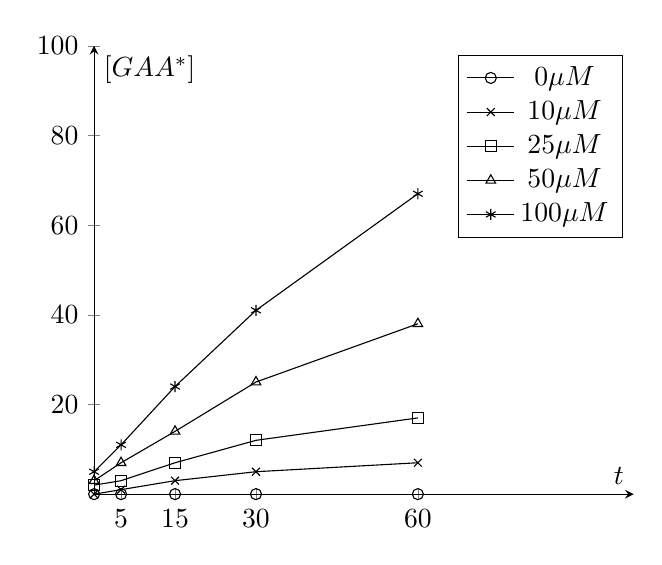
\begin{tikzpicture}
					\begin{axis}[axis lines=middle, xmin=0, xmax=100, ymin=0, ymax=100,samples=100, xtick={5, 15, 30, 60}, xlabel={$t$}, ylabel={$[GAA^*]$}]
					\addplot[
					scatter,
					point meta=explicit symbolic,
					scatter/classes={
						a={mark=o,draw=black},
						b={mark=x, draw=black},
						c={mark=square,draw=black},
						d={mark=triangle,draw=black},
						e={mark=asterisk,draw=black}}
					]
					table [meta=label, col sep=comma, row sep=crcr]{
						x, y, label, err\\
						0, 0, a, 1\\
						5, 0, a, 2\\
						15, 0, a, 3\\
						30, 0, a, 4\\
						60, 0, a, 5\\
					};
					\addplot[
					scatter,
					point meta=explicit symbolic,
					scatter/classes={
						a={mark=o,draw=black},
						b={mark=x, draw=black},
						c={mark=square,draw=black},
						d={mark=triangle,draw=black},
						e={mark=asterisk,draw=black}}
					]
					table [meta=label, col sep=comma, row sep=crcr]{
						x, y, label\\
						0, 0, b\\
						5, 1, b\\
						15, 3, b\\
						30, 5, b\\
						60, 7, b\\
					};
					\addplot[
					scatter,
					point meta=explicit symbolic,
					scatter/classes={
						a={mark=o,draw=black},
						b={mark=x, draw=black},
						c={mark=square,draw=black},
						d={mark=triangle,draw=black},
						e={mark=asterisk,draw=black}}
					]
					table [meta=label, col sep=comma, row sep=crcr]{
						x, y, label\\
						0, 2, c\\
						5, 3, c\\
						15, 7, c\\
						30, 12, c\\
						60, 17, c\\
					};
					\addplot[
					scatter,
					point meta=explicit symbolic,
					scatter/classes={
						a={mark=o,draw=black},
						b={mark=x, draw=black},
						c={mark=square,draw=black},
						d={mark=triangle,draw=black},
						e={mark=asterisk,draw=black}}
					]
					table [meta=label, col sep=comma, row sep=crcr]{
						x, y, label\\
						0, 3, d\\
						5, 7, d\\
						15, 14, d\\
						30, 25, d\\
						60, 38, d\\
					};
					\addplot[
					scatter,
					point meta=explicit symbolic,
					scatter/classes={
						a={mark=o,draw=black},
						b={mark=x, draw=black},
						c={mark=square,draw=black},
						d={mark=triangle,draw=black},
						e={mark=asterisk,draw=black}}
					]
					table [meta=label, col sep=comma, row sep=crcr]{
						x, y, label\\
						0, 5, e\\
						5, 11, e\\
						15, 24, e\\
						30, 41, e\\
						60, 67, e\\
					};
					
					
					
					\legend{$0\mu M$,$10\mu M$,$25\mu M$,$50\mu M$,$100\mu M$};
					
					\end{axis}
					\end{tikzpicture}
				}
			\end{figure}
	
	
	\column{.45\textwidth}
\begin{figure}
	\center
	\resizebox{.9\textwidth}{!}{
		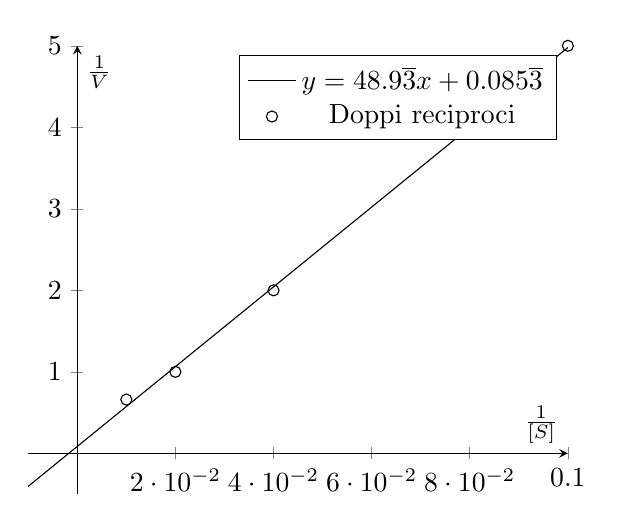
\begin{tikzpicture}
		\begin{axis}[axis lines=middle, xmin=-0.01, xmax=0.1, ymin=-0.5, ymax=5,domain=-0.1:0.5,samples=100, xlabel={$\frac{1}{[S]}$}, ylabel={$\frac{1}{V}$}]
		\addplot[black]{48.9333*x + 0.0853333};
		\addplot[
		scatter,
		only marks,
		point meta=explicit symbolic,
		scatter/classes={
			a={mark=o,draw=black}}
		]
		table [meta=label, col sep=comma, row sep=crcr]{
			x, y, label\\
			0.1, 5, a\\
			0.04, 2, a\\
			0.02, 1, a\\
			0.01, 0.66, a\\
		};
		
		\legend{$y = 48.9\overline{3}x + 0.085\overline{3}$,Doppi reciproci};
		
		\end{axis}
		\end{tikzpicture}
	}
\end{figure}

\end{columns}
	
\end{frame}

\begin{frame}
	\frametitle{Red Cell Loader}
	\framesubtitle{Esperimenti \emph{in vitro}: sintesi di creatina da parte degli RBC ingegnerizzati}
	
	\begin{columns}[t]
		\column{.3\textwidth}
		\begin{block}{RBC non ingegnerizzati \phantom{aaaaaaaaaaaaaaaaaaaaa}}
			\resizebox{\textwidth}{!} {
				\begin{tabular}{| c | c | c |}
					\hline
					Tempo (ore) & $[GAA]\ (\mu M)$ & $[Cr]\ (\mu M)$ \\
					\hline
					0 & 0.13 & 59.80\\
					\hline
					1 & 0.15 & 72.20\\
					\hline
					2 & 0.16 & 75.25\\
					\hline
					3 & 0.20 & 75.86\\
					\hline
					20 & 0.27 & 76.31\\
					\hline
				\end{tabular}
			}
		\end{block}
		\column{.3\textwidth}
		\begin{block}{250 $\mu g/ml$ di GAMT e 25 $\mu M$ di SAM}
			\resizebox{\textwidth}{!} {
				\begin{tabular}{| c | c | c |}
					\hline
					Tempo (ore) & $[GAA]\ (\mu M)$ & $[Cr]\ (\mu M)$ \\
					\hline
					0 & 2.61 & 66.01\\
					\hline
					1 & 3.10 & 61.90\\
					\hline
					2 & 4.62 & 63.37\\
					\hline
					3 & 5.11 & 67.50\\
					\hline
					20 & 5.26 & 59.31\\
					\hline
				\end{tabular}
			}
		\end{block}
		\column{.3\textwidth}
		\begin{block}{250 $\mu g/ml$ di GAMT e 125 $\mu M$ di SAM}
			\resizebox{\textwidth}{!} {
				\begin{tabular}{| c | c | c |}
					\hline
					Tempo (ore) & $[GAA]\ (\mu M)$ & $[Cr]\ (\mu M)$ \\
					\hline
					0 & 7.32 & 66.32\\
					\hline
					1 & 10.52 & 64.55\\
					\hline
					2 & 13.87 & 65.87\\
					\hline
					3 & 12.18 & 61.58\\
					\hline
					20 & 15.13 & 59.88\\
					\hline
				\end{tabular}
			}
		\end{block}
		
	\end{columns}
	
\end{frame}
